\documentclass{jsarticle}

 \usepackage{ascmac}
 \usepackage{graphicx}
 \usepackage[dvipdfmx]{color}
 \usepackage{amssymb,amsmath,amsthm}
 \usepackage{graphics}
 \usepackage{fancybox, tcolorbox}
 \tcbuselibrary{raster,skins, breakable}
 \usepackage{nccmath}
 \usepackage{tikz}
 \usetikzlibrary{intersections, calc, cd}
 \usepackage{bm}
 \usepackage[italicdiff]{physics}
 \usepackage{titlesec}
 \usepackage{mathtools}
 \usepackage{enumerate}
 \usepackage{float}

 \newcommand{\myproof}[1]{
  \begin{tcolorbox}[
    empty,top = -2pt, breakable = true,
    underlay = {
      \draw[line width = 5pt, color = teal] (frame.north west) -- (frame.south west);
      },
    underlay unbroken = {
      \fill (frame.south east) -- ([xshift = -5pt]frame.south east) --([xshift = -5pt, yshift = -7pt]frame.south east) -- ([yshift = -7pt]frame.south east) -- cycle;
    },
    underlay last = {
        \fill (frame.south east) -- ([xshift = -5pt]frame.south east) --([xshift = -5pt, yshift = -7pt]frame.south east) -- ([yshift = -7pt]frame.south east) -- cycle;
      }
    ]
    {\it Proof.}

    {#1}
  \end{tcolorbox}
 }

 \numberwithin{equation}{section}
 \setcounter{tocdepth}{3}

\theoremstyle{definition}
\newtheorem{dfn}{定義}[section]
\newtheorem{exa}{例}[section]
\newtheorem{thm}[dfn]{定理}
\newtheorem{prop}[dfn]{命題}
\newtheorem{note}[dfn]{注意}
\newtheorem{prob}[dfn]{問}
\newtheorem{coro}[dfn]{系}

\newcommand{\ave}[1]{\langle #1 \rangle}

\usepackage{fancyhdr}
\pagestyle{fancy}
    \lfoot{}
    \cfoot{\thepage}
    \rfoot{}

\begin{document}
最後に Reduced VSR をヒト赤血球(RBC)に適用する.RBCは解糖系を通してグルコースをATPに代謝し,細胞膜のアクティブな振動を引き起こし,それに伴いエントロピーが生成する.\\
この論文では3つの方法でRBCの実験を行った.1つは異なる強度の光トラップにより,膜に非特異的に結合したビーズを使ってRBCを機械的に引き延ばす方法.2つ目は先行研究(11)のデータを用いてRBC膜を機会的にセンシングする方法.3つ目は振動セグメントの追跡により,膜の輪郭の揺らぎを測定する方法である.\\
ここでは図 \ref{rbc_1} のように,見えない変数 $y(t)$ を設定した2層モデルを検討した.

\begin{figure}[H]
  \begin{center}  
  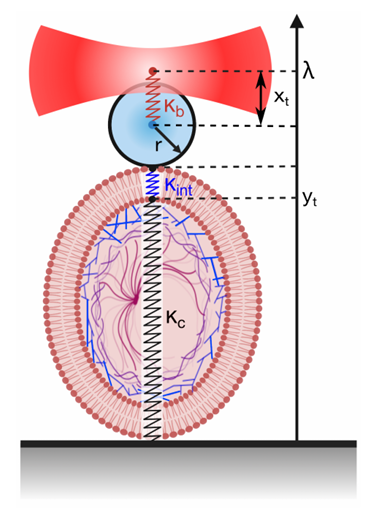
\includegraphics[width=5cm]{rbc.png}  
  \end{center}
  \caption{RBCモデル}
  \label{rbc_1}
\end{figure}

$x(t)$は測定することができる変数である.これらの変数はつぎの方程式を満たす.
\begin{equation}
  \dot{x}(t) = \mu_x (-k_b x(t) - k_{int}(x(t) - y(t)) + C_1) + \sqrt{2D_x} \eta^x (t) 
\end{equation}
\begin{equation}
  \dot{y}(t) = \mu_y (-k_c y(t) + k_{int}(x(t) - y(t)) + f^a (t) + C_2) + \sqrt{2D_y} \eta^y (t) 
\end{equation}
ここで $k_{i}$ は実効的な力の定数であり,$\mu_{i}, \eta_{i}$は移動度とホワイトノイズである.また,$C_i$は定数,$D_i$は $D_i = k_B T \mu_i$ である.$f^a (t)$は確率的なアクティブ力であって,つぎの関係を満たす.
\begin{equation}
  \dot{f}^a (t) = - \frac{f^a (t)}{\tau_a} + \sqrt{\frac{2 \epsilon^2}{\tau_a}} \eta^f (t)
\end{equation}
ただし,
\begin{equation}
  \ave{\eta^f (t) \eta^f (t')} = \delta (t - t')
\end{equation}
以上の方程式を用いて,相関関数($t = 0$)を計算すると,つぎのようになる.

\begin{figure}[H]
  \begin{center}  
  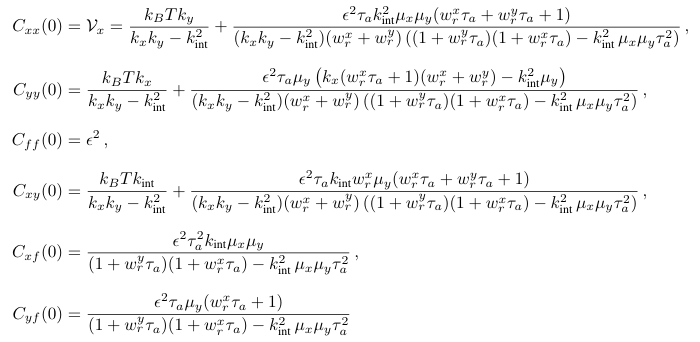
\includegraphics[width=8cm]{rbc_2.png}  
  \end{center}
\end{figure}

ただし,$k_x = k_b + k_{int}, k_y = k_c + k_{int}, k_x \mu_y = w^x_r, k_y \mu_y = w^y_r$ である.
これらを持ちいて時刻 $t$ における相関関数を計算し,Reduced-VSRを考える.

\begin{equation}
  \sigma_{th} = \frac{\mu_y \epsilon^2 (1 + w^x_r \tau_a)}{(1+w^y_r \tau_a)(1 + w^x_r \tau_a) - k_{int}^2 \mu_x \mu_y \tau^2_a}
\end{equation}

% 図4. RBCにおける簡略化VSRの適用例。
% (A) OT伸張実験。RBCを引き伸ばした映像と接触面積推定の概略図(左);(右)高(青)、中(オレンジ)、低(赤)のトラップ剛性における3つのビーズ位置トレース。
% (B) OTセンシング実験。実験装置の配置図(左)と健康なRBC(赤)および受動的なRBC(青)のビーズ位置トレース(右)。
% (C) 超高速OM測定:健康なRBC(上段の画像)および細胞輪郭上の3つの選択ピクセル(50 nm × 50 nm)の位置トレース(右)。高(赤)、中(黄)、低(緑)の分散Vx。受動的なRBC(下段の画像)と細胞輪郭上の3つの選択ピクセルのトレース(青、右)。右の画像には細胞輪郭上の色分散マップも示される。色バーは分散レベルを示し、赤が最高、青が最低を表す。
% (D) OT伸張におけるsと位置分散Vxの測定。健康なRBCにおいてトラップ剛性kbを高(右端:5 × 10² pN/nm)から低(左端:7 × 10⁴ pN/nm)に変化させた場合。
% (E) 健康な(赤い記号)および受動的な(青い記号)RBCのOTセンシングのs測定。
% (F) OM測定で健康なRBC(丸印)および受動的なRBC(菱形)の赤道細胞輪郭に沿った色付きsマップ。放射距離は任意単位のsを表し、オレンジ色の曲線はsの平滑化プロファイル。
% (G) (F)のRBCにおけるsとVxの散布図。これらは部分的に逆相関している。オレンジの丸印はVxの50 nm²ウィンドウで平均化したs値。
% (H) 細胞輪郭に沿ったsと位置xの空間相関関数。
% (I) OT伸張におけるsRBCの値と熱量測定による推定値の比較。暗赤色(明赤色)のバーは最低(最高)トラップ剛性を示す。


\end{document}